\documentclass[10pt,a4paper,twoside]{report}
\usepackage[utf8]{inputenc}
\usepackage{amsmath}
\usepackage{amsfonts}
\usepackage{amssymb}
\usepackage{graphicx}
\usepackage{fancyhdr}
\usepackage{listings}
\renewcommand{\bibname} {REFERENCES}
\usepackage[T1]{fontenc}
\usepackage{lmodern}
\usepackage{geometry}
\usepackage{textcomp}
\usepackage{afterpage}
\newcommand\blankpage{
	\null
	\thispagestyle{empty}
	\addtocounter{page}{-1}
	\newpage}

\title{
\vspace{-3.4cm}
\begin{center}
%{\Large First Progress Report}\\
{\Large {\textbf{INTERMEDIATE REPORT}}  }\\
{\Large {\textbf{ON}}}\\
{\textbf{\Large{{GUIDANCE PERFORMANCE ANALYSIS FOR   }}}}\\
\vspace{0.01 cm}
{\textbf{\Large{{BLIND NAVIGATION SYSTEM USING  }}}}\\
\vspace{0.01 cm}
{\textbf{\Large{{NEURAL LEARNING IMAGE RECOGNITION}}}}\\
\vspace{0.2cm}
\begin{small}
 Submitted By :
 \end{small}
\begin{center}
\begin{large}
{AJITHKUMAR AK\hspace{13mm}EPAMEIT003}\\
{AKHIL A{\hspace{32mm}}EPAMEIT004}\\
{ARAVIND RAVINDRAN\hspace{3mm}EPAMEIT016}\\
{JITHIN S\hspace{32mm}EPAMEIT033}\\
{KIRAN TS\hspace{29mm}EPAMEIT034}\\
\end{large}
\end{center}
{\Large Guided By : }
{\textbf{\large Mr. RANJITH K }}\\
\begin{small}
(Asst.Prof. Department of Information Technology)
\end{small}
\end{center}
\vspace{0.05cm}
\begin{figure}[htbp]
\begin{center}
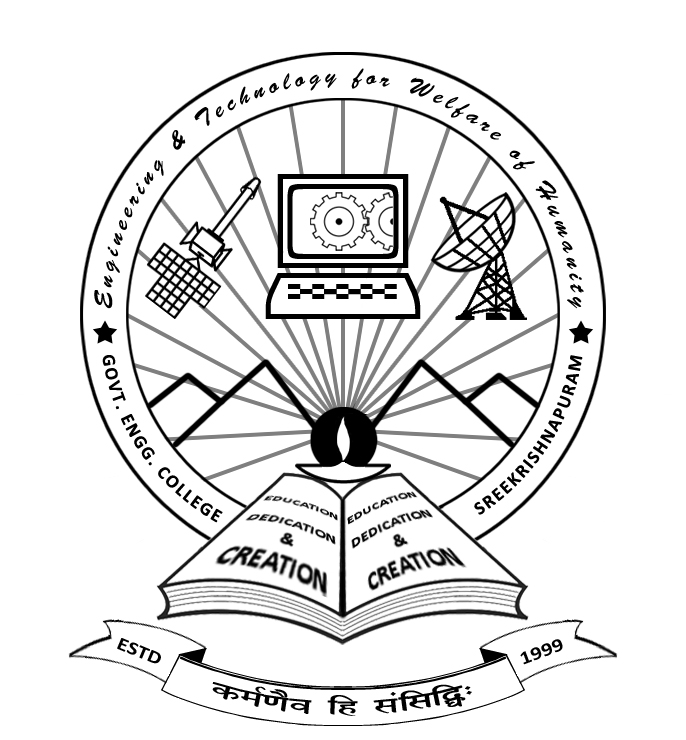
\includegraphics[scale=0.2]{emblem1.jpg}
\end{center}
\end{figure}
\begin{center}
%\vspace{0.25 cm}
{\Large Department of Information Technology} \\
%\vspace{0.015 cm}
{\Large Government Engineering College, Sreekrishnapuram}\\
%\vspace{0.015 cm}
{\large PALAKKAD - 678633}\\
%\vspace{0.25cm}
%{\large February, 2014}
%\tableofcontents
\end{center}
}
\begin{document}
\pagenumbering{gobble}
\maketitle
\cleardoublepage
\newpage

\pagenumbering{roman}
\setcounter{page}{0}
\newpage
\begin{center}
\begin{large} 
2015-2016\\
\vspace{2pt}
\textbf{ GOVERNMENT ENGINEERING COLLEGE }\\
\vspace{5pt}
\textbf{ SREEKRISHNAPURAM}\\
\vspace{5pt} 
\textbf{ PALAKKAD-678 633}   \\ 
\end{large}

 \vspace{8pt}
 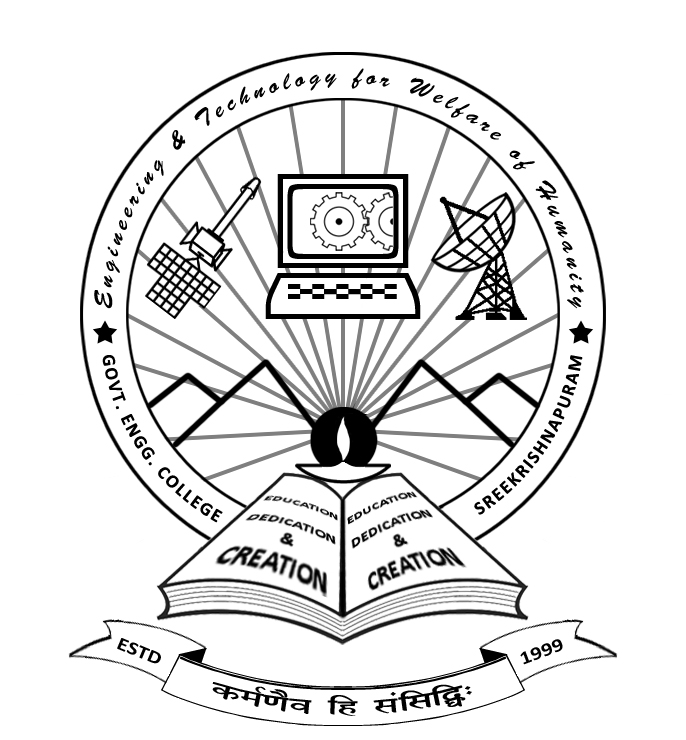
\includegraphics[scale=0.2]{emblem1.jpg}
 
 \vspace{8pt}
 { \bf  DEPARTMENT OF\\ INFORMATION TECHNOLOGY}\\
 \vspace{17pt} 
 \begin{LARGE}
 \textsc{CERTIFICATE}
 \end{LARGE}

\end{center} \hspace{10pt}
 This is to certify  that  the  Main project  report entitled  as  {\bf GUIDANCE PERFORMANCE ANALYSIS FOR BLIND NAVIGATION SYSTEM USING NEURAL LEARNING IMAGE RECOGNITION }  submitted by AJITHKUMAR AK(EPAMEIT003), AKHIL A(EPAMEIT004), ARAVIND RAVINDRAN(EPAMEIT016), JITHIN S(EPAMEIT033), KIRAN TS(EPAMEIT034) to the {\bf Department   Of   Information Technology}, Government Engineering College, Sreekrishnapuram, Palakkad, in partial fulfilment of the requirement for the award of B.Tech Degree in Information Technology is a bonafide record of the work carried out by him.
\newline
\newline
\textbf{Co-ordinator}\hspace{9.9cm}\textbf{Guide}
\newline
Asst.Prof. Vinayachandran.K.K \hspace{6.2cm}Mr.Ranjith K
\\
Asst.Prof. Sreedivya RS\\
Miss Geethu Mary George 
\newline
\\
 \begin{center}
 \textbf{Head of the Department}
 \\
Mrs.Dhanya 
\end{center}

\begin{flushleft}

{\bf Place}: Sreekrishnapuram
\newline 
{\bf Date}:\hspace{.1cm}
\end{flushleft}


\newpage
\pagenumbering{gobble}
\blankpage
\newpage
\pagenumbering{roman}
\setcounter{page}{0}
\begin{center}
\begin{Large}
\textbf{ACKNOWLEDGEMENT}
\end{Large}
\end{center}
\paragraph{ }
We are pleased to acknowledge \textbf{Dr.S.Radhakrishnan} principal Govt. Engineering College Sreekrishnapuram for his inspiration throughout the project. We are deeply indebted to \textbf{Prof. Dhanya KM} Head of the Department of Information Technology Government Engineering College Sreekrishnapuram for providing permission and availing all required facilities for undertaking the project in a systemic way. We extend our sincere thanks to \textbf{Asst.prof. Ranjith K} Department of Information Technology Government Engineering college Sreekrishnapuram  who continuously helped us throughout the project and without his guidance, this project would have been an uphill task. We are also grateful to \textbf{Mr. Vinayachandran K K} ( Assistant Professor in Information Technology), \textbf{Mrs.
Sree Divya R S} (Assistant Professor in Information Technology) and  \textbf{Miss. Geethu Mary George} ( Assistant Professor in Information Technology), our project co-ordinators Department of Information Technology Government Engineering College Sreekrishnapuram for their exemplary guidance, monitoring and constant encouragement throughout the project. We are also grateful to other faculty and non-faculty members who co-operated with us regarding some issues.
\begin{flushright}
AJITHKUMAR AK\\
AKHIL A\\
ARAVIND RAVINDRAN\\
JITHIN S\\
KIRAN TS
\end{flushright}
\newpage
\pagenumbering{roman}
\setcounter{page}{0}
\newpage
\pagenumbering{gobble}
\blankpage
\begin{center}
\begin{Large}
\textbf{ABSTRACT}
\end{Large}
\end{center}
\paragraph{ }
Blind people are facing some problems to travel without a guide. Proper and affordable navigating and identification systems are not available for them. So our aim is to create a system which helps the blind person to navigate and identify people in-front of them with very less expense. This make blind people to navigate with the help of a Smartphone and a system equipped with an ultrasonic sensors and a camera. The blind can only get perceptive and audio information, which bring them huge barriers to action. Mobile devices could provide the blind great help. Here the project presents a system which uses neural network for face recognition, which widely provides the blind user to identify the person in-front of him. Also the  project provides a system to navigate the blind, detect the obstacles in-front of him and provide instructions for easier navigation.
\begin{itemize}
\item KEYWORDS
\begin{itemize}
\item NEURAL NETWORK
\item MULTI LAYER PERCEPTRON
\item BACK PROPAGATION
\item SIGMOID FUNCTION

\end{itemize}
 \pagenumbering{gobble}
 \newpage
\blankpage

\end{itemize}
 

%===========================================================
\pagenumbering{roman}
\setcounter{page}{0}

\tableofcontents
%========================================================
\listoffigures
%========================================================
\newpage
\begin{LARGE}
\textbf{List of Abbreviation}
\end{LARGE}
\begin{small}


\begin{itemize}
\item GPS \hspace{4mm}  :GLOBAL POSITIONING SYSTEM
\item GIS \hspace{5mm} :GLOBAL INFORMATION SYSTEM
\item SDK \hspace{3.6mm} :SOFTWARE DEVELOPMENT KIT
\item API  \hspace{6mm}:APPLICATION PROGRAM INTERFACE
\item ETA \hspace{3.6mm} :ELECTRONIC TRAVEL AID
\item QOS  \hspace{4.7mm}:QUALITY OF SERVICE

\end{itemize}
\end{small}




\chapter{INTRODUCTION}
\pagenumbering{arabic}

\pagestyle{fancy}
\rhead{\thepage}
\chead{}
\lhead{\textit{GUIDANCE PERFORMANCE ANALYSIS FOR BLIND NAVIGATION SYSTEM USING NEURAL LEARNING IMAGE RECOGNITION}}

\lfoot{\textit{Dept.Of Information Technology, Govt.Engg.College,Sreekrishnapuram }}
\cfoot{}
\rfoot{}
\renewcommand{\headrulewidth}{0.4pt}
\renewcommand{\footrulewidth}{0.4pt}

\paragraph{ }According to survey done India is now home to the world’s largest number of blind people. Of the 37 million people across the globe who are blind, over 15 million are from India. So in India blindness is the biggest problem. The leading causes of blindness are cataract, uncorrected refractive errors, glaucoma, and macular degeneration. Our goal is to create a portable, self-contained system that will allow visually impaired individuals to travel through familiar and unfamiliar environments without the assistance of guides and to recognize persons in front of the blind with the help of a smartphone. We uses a technology called Neural Network for image recognition. A key priority of this system is to meet the users navigation needs while ensuring low cost and portability embedded it with a Smartphone. The camera of the smartphone  is used to take real time images in front of the user, detect faces, process these faces using Neural Network and analyze it and finally recognize the face in front of him. A database consisting of images  is compared with the images captured at real time and suitable results is obtained.
\section{PROBLEM DEFINITION}
\paragraph{ } The blind people in our society are facing problems during their navigation. There are no proper navigation systems that help blind people effectively. One of the disadvantage about the existing navigation systems are they are not affordable for the common user. A key priority of our system is to meet the users navigation needs while ensuring low cost and portability embedded it with a Smartphone.  The existing systems cannot identify objects and people in front of the person. The project described here develops a navigation system that makes use of GPS, voice, ultrasonic sensor for obstacle detection and includes face detection system using neural network.
\newpage
\section{SCOPE}
\paragraph{ }The existing systems cannot identify objects and people in front of the person. The project aims to create a low cost system which uses the Smartphone for real time images and identifying persons in front of the user. The images are analyzed and suitable results are obtained using Neural Network technology. Apart from this the person can navigate easily with the help of ultra-sonic sensors and the associated devices with the user.

%=====================================================================================================
\chapter{PREVIOUS WORKS}

\section{THERMAL CAMERA}
\paragraph{ }A different form of taking input data for face recognition is by using thermal cameras, by this procedure the cameras will only detect the shape of the head and it will ignore the subject accessories such as glasses, hats, or make up. A problem with using thermal pictures for face recognition is that the databases for face recognition is limited. Diego Socolinsky, and Andrea Selinger (2004) research the use of thermal face recognition in real life, and operation sceneries, and at the same time build a new database of thermal facial images. The research uses low-sensitive, low-resolution ferro-electric electrics sensors that are capable of acquire long wave thermal infrared (LWIR). The results show that a fusion of LWIR and regular visual cameras has the greater results in outdoor probes. Indoor results show that visual has a 97.05 percentage accuracy, while LWIR has 93.93, and the Fusion has 98.40, however on the outdoor proves visual has 67.06, LWIR 83.03, and fusion has 89.02. The study used 240 subjects over the period of 10 weeks to create the new database. The data was collected on sunny, rainy, and cloudy days.
\section{SKIN  TEXTURE ANALYSIS}
\paragraph{ }It uses the visual details of the skin, as captured in standard digital or scanned images. This technique, called skin texture analysis, turns the unique lines, patterns, and spots apparent in a person’s skin into a mathematical space.
\section{LEARNING BASED COMPUTER VISION WITH INTEL OPEN SOURCE COMPUTER VISION LIBRARY}
\paragraph{ }The rapid expansion of computer processing power combines with the rapid development of digital camera capability has resulted in equally rapid advances in computer vision capability and use. Intel has long been at the forefront of enabling this advance on the computer hardware and software side. Computer Vision software is supported by the free Open Source Computer Vision Library (OpenCV) that optionally may be highly optimized by loading the commercial Intel Integrated Performance primitives (IPP). IPP now automatically supports OpenCV with no need to change  or even recompile the user’s source code. This functionality enables development groups to deploy vision and provides basic infrastructure to experts in vision.

\section{FACE RECOGNITION SOFTWARE}
\paragraph{ }A facial recognition system is a computer application capable of identifying or verifying a person from a digital image or a video frame from a video source. One of the ways to do this is by comparing selected facial features from the image and a facial database.
\paragraph{ }Main face recognizing softwares are:
\subsection{iPHOTO}
\paragraph{ }iPhoto was a digital photograph manipulation software application developed by Apple Inc. It was included with every Macintosh personal computer from 2002 to 2015, when it was replaced with Apple's Photos application. Originally sold as part of the iLife suite of digital media management applications, iPhoto can import, organize, edit, print and share digital photos.
\subsection{OpenCV}
\paragraph{ }OpenCV (Open Source Computer Vision) is a library of programming functions mainly aimed at real-time computer vision, originally developed by Intel research center in Nizhny Novgorod (Russia), later supported by Willow Garage and now maintained by Itseez.[1]The library is cross-platform and free for use under the open-source BSD license.
\subsection{PICASSA}
\paragraph{ }Picasa is an image organizer and image viewer for organizing and editing digital photos, plus an integrated photo-sharingwebsite, originally created by a company named Lifescape (which at that time may have resided at Idealab) in 2002. In July 2004, Google acquired Picasa from Lifescape and began offering it as freeware "Picasa" is a blend of the name of Spanish painter Pablo Picasso, the phrase mi casa (Spanish for "my house") and "pic" for pictures.

\section{CONVENTIONAL ELECTRONIC
TRAVEL AIDS}
\paragraph{ }In the past three decades several electronic travel aids (ETAs) were introduced that
aimed at improving their blind users’ mobility in terms of safety and speed. The C-5
Laser Cane – was introduced in 1973 by Benjamin et al. [1973]. It is based on optical
triangulation with three laser diodes and three photo-diodes as receivers. The Laser
Cane can detect obstacles at head-height, drop-offs in front of the user, and obstacles
up to a range of 1.5 m or 3.5 m ahead of the user.
\begin{itemize}
\item The Mowat sensor : is a commercially available [WORMALD] hand-held ultrasonicbased device that informs the user of the distance to detected objects by means of
tactile vibrations.The frequency of the vibration is inversely proportional to the distance
between the sensor and the object.
\item The Nottingham Obstacle Detector (NOD) : is a hand-held sonar device that provides
an auditory feedback that indicates eight discrete levels of distance by different
musical tones.
\item The Path Sounder : is one of the earliest ultrasonic travel aids. Two ultrasonic transducers are mounted on a board that the user wears around the neck, at chest height. This
unit provides only three discrete levels of feedback (series of clicks), coarsely indicating
distances to an object.
\item The Binaural Sonic Aid (Sonicguide) : Comes in the form of a pair of spectacle frames,
with one ultrasonic wide-beam transmitter mounted between the spectacle lenses and
one receiver on each side of the transmitter [Kay, 1974]. Signals from the receivers are
frequency shifted and presented separately to the left and right ear. The resulting interaural
amplitude difference allows the user to determine the direction of an incident echo
and thus of an obstacle. The distance to an object is encoded in the frequency of the
demodulated low-frequency tone. 

\end{itemize}

%========================================================================================================
\newpage
\blankpage
\chapter{EXPERIMENTAL SETTINGS}
\section{SYSTEM REQUIREMENTS}
\begin{itemize}
\item Microsoft® Windows® 8.1/10 (32 or 64-bit).
\item 2 GB RAM minimum.
\item 400 MB hard disk space.
\item At least 1 GB for Android SDK, emulator system images, and caches.
\item 1280 x 800 minimum screen resolution.
\item Java Development Kit (JDK) 7.
\item Optional for accelerated emulator: Intel® processor with support for Intel® VT-x, Intel® EM64T (Intel® 64), and Execute Disable (XD) Bit functionality.

\end{itemize}
\section{SOFTWARE SECTION}
\begin{itemize}
\item Android SDK version 18 or higher: It is the software development kit developed
by android which helps developers to create software.
\item Google API: It is the application programming interface provided by google in
which developers can interface their application with google services like google
map etc.
\item TTS: It is another application service provided by the android which helps to
convert text into speech.
\item Android studio 5.0: It is the SDK which helps android programming easier.
\item OpenCV.
\end{itemize}
\section{HARDWARE SECTION}
\begin{itemize}
\item Arduino UNO : It is micro-controller which is used in the hardware part which
receives information from ultrasonic sensor and sends this data to a Smartphone
via a Bluetooth module attached to it.
\item Ultrasonic sensor (HC-SR04): It is an ultrasonic sensor which detects obstacles
in-front of the user and gives information to the micro-controller attached to it.
\item Bluetooth module (HC-06): It is connected to the micro-controller, sends instructions
to the Smartphone whenever obstacle is detected in-front of the user.
\item Smartphone: Any Smartphone which has android OS can be used which has access
to the Google services and have a compass inbuilt in it.


\end{itemize}

%=======================================================================================================
\chapter{MATHEMATICAL BACKGROUND}

\section{PERCEPTRON}
\paragraph{ }In machine learning, the perceptron is an algorithm for supervised learning of binary classifiers: functions that can decide whether an input (represented by a vector of numbers) belongs to one class or another.[2] It is a type of linear classifier, i.e. a classification algorithm that makes its predictions based on a linear predictor function combining a set of weights with the feature vector. The algorithm allows for online learning, in that it processes elements in the training set one at a time.\\
\begin{center}
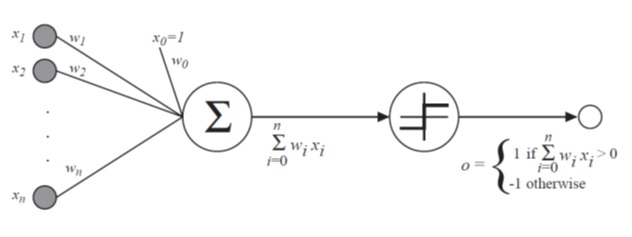
\includegraphics[scale=.75]{per.jpg}
\end{center}
It takes the inputs:
\begin{itemize}
\item $\sum_{i=0}^{n}w_ix_i =w_0x_0+w_1x_1+....+w_nx_n  $
\item $w_0$ denotes a threshold value
\item $x_0$ always 1
\end{itemize}
It outputs 1, if the result is greater than 1, otherwise -1
\paragraph{ }It can be used also for non-separable data sets, where the aim is to find a perceptron with a small number of misclassifications. However, these solutions appear purely stochastically and hence the pocket algorithm neither approaches them gradually in the course of learning, nor are they guaranteed to show up within a given number of learning steps.
\paragraph{ }Perceptron trainning rule
\begin{itemize}
\item uses thresholded unit
\item converges after a finite number of iterations
\item output hypothesis classifies training data perfectly
\item linearly separability necessary
\end{itemize}
\section{MULTILAYER PERCEPTRON }
\paragraph{ }It can be used also for non-separable data sets, where the aim is to find a perceptron with a small number of misclassifications. However, these solutions appear purely stochastically and hence the pocket algorithm neither approaches them gradually in the course of learning, nor are they guaranteed to show up within a given number of learning steps.
\begin{center}
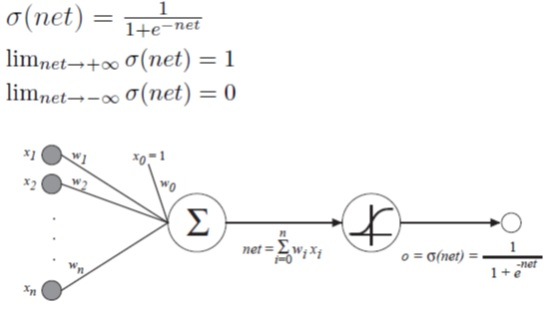
\includegraphics[scale=.75]{mlp.jpg}
\end{center}

\section{BACK PROPAGATION}
\paragraph{ }Learning occurs in the perceptron by changing connection weights after each piece of data is processed, based on the amount of error in the output compared to the expected result. This is an example of supervised learning, and is carried out through back propagation, a generalization of the least mean squares algorithm in the linear perceptron.

%=======================================================================================================
\chapter{EXPECTED INPUT}
\begin{itemize}
\item Training inputs
\begin{enumerate}
\item Faces
\item Non faces
\item Desired faces
\end{enumerate}

\end{itemize}
\begin{figure}[htpb]
\begin{center}
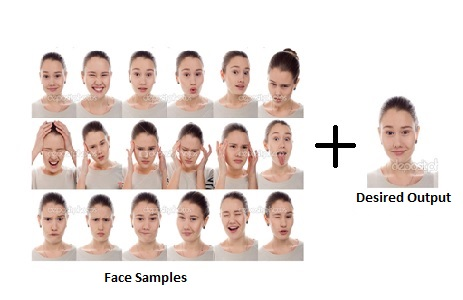
\includegraphics[scale=1]{input.jpg}
\caption{Expected inputs}
\end{center}
\end{figure}
\newpage
\begin{itemize}
\item Real time inputs
\begin{center}
\begin{figure}[htpb]
\center 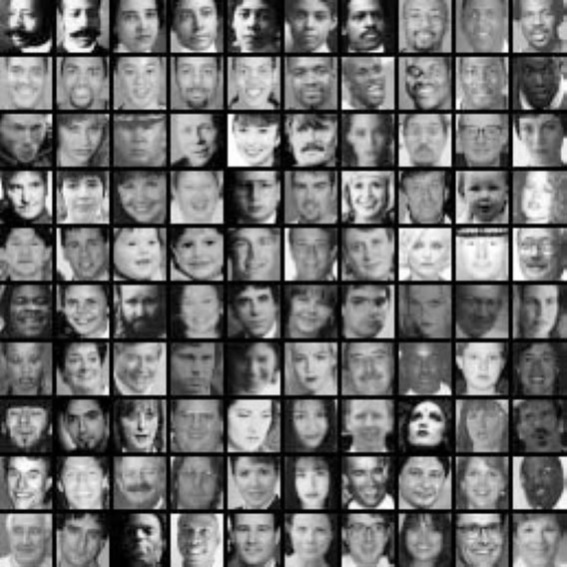
\includegraphics[scale=.5]{real}
\caption{Real time Inputs}
\end{figure}


\end{center}
\end{itemize}

%=======================================================================================================
\chapter{EXPECTED OUTPUT}
\begin{itemize}
\item Train Outputs
\begin{enumerate}
\item	The facial features converted to normalized values and these values stored in database
\item Fully trained neural network which is ready for real time testing.

\end{enumerate}
\end{itemize}



\begin{itemize}
\item Real Time Output
\begin{enumerate}
\item If the person already in database then identify the person
\item If person not in database ask if want to add to database

\end{enumerate}

\end{itemize}
\begin{figure}[htpb]

\begin{center}
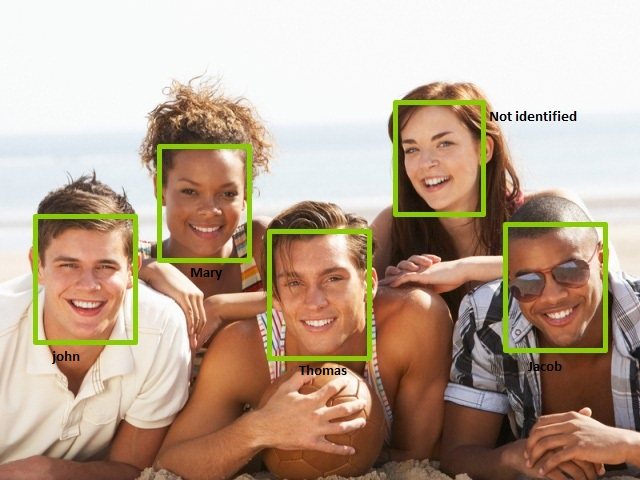
\includegraphics[scale=.5]{out}
\caption{Expected Output }
\end{center}

\end{figure}

%=======================================================================================================
\newpage
\blankpage
\chapter{ANALYSIS}
\paragraph{ }The result during our testing procedure shows that the application developed by the concept of Neural Network and adaboost has significant detection rate. We have used the existing open cv library methods for sample testing and it shows high performance rate. 
\begin{figure}[htpb]
\begin{center}

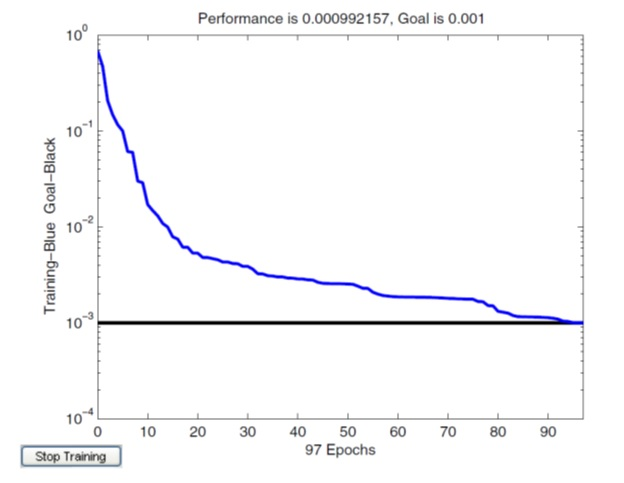
\includegraphics[scale=.5]{performance}
\caption{Performance analysis}


\end{center}
\end{figure}
%=======================================================================================================
\newpage
\blankpage
\chapter{CONCLUSION AND FUTURE SCOPE}
\paragraph{ }The project provides a system for Blind person to identify the people in-front of him using Neural Learning image recognition. Blind people can easily navigate and identify individuals. This also provide voice instructions for navigation through the Smartphone and ultrasonic sensors detect the obstacles and instructs the user through the smart phone paired by Bluetooth module. Most systems that have been developed, so far lack the kind of dynamic interaction and adaptability to changes that our system provides to the user. The Google Map provides all the instructions for navigation.
\paragraph{ }In future this project can be enhanced for character recognition, object recognition and navigation can be done using camera instead of ultrasonic sensors.
%=======================================================================================================
\textbf{\newpage
\blankpage}
\chapter{ACTIVITY BLOCK DIAGRAM}
\begin{small}
\begin{tabular}{|p{1cm}|p{2cm}|p{4.3cm}|p{4.3cm}|} 
\hline 
Sl.No.& Date & Work intended &  Actual Work done  \\ 
\hline 
1&  14/7/2015-24/7/2015 &  To find a problem for main project. & Find out a problem of face recognition embedded with blind navigation.
\\   								              
\hline 
2& 	25/7/2015-07/08/2015 & Familiarize with the details of the project Topic & Study Various fields related to the topic and presented the summary
\\
\hline
3 &  14/8/2015-16/09/2015 & Works for submitting slides for each reference paper  & Submitted slides for each reference paper
\\
\hline 
4 & 29/9/2015-30/10/2015  &Work for submitting literature review &   Submitted literature review
Familiarized neural network concept including Multilayer perceptron concept
\\
& &To familiarize the concept of Neural network&
\\
\hline 
%\end{tabular}


%\begin{tabular}{|p{1cm}|p{2cm}|p{4cm}|p{4cm}|}


5 & 20/11/2015-14/12/2015 & Started coding in Android studio to create the front end &Created the front end of the app  
\\
\hline 
6 & 15/12/2015-25/12/2015 &Work for 1st presentation to prepare slides &1st presentation slides were prepared
 \\   	
\hline 
7 & 26/12/2015-08/01/2016& 1st presentation preparation& First presentation was conducted
\\
\hline
\end{tabular} 
\end{small}
%=======================================================================================================
\addcontentsline{toc}{chapter}{REFERENCES}
\vspace{2pt}
\begin{thebibliography}{10}

\bibitem{key1}Zulhadi Zakaria, Nor Ashidi Mat Isa, and Shahrel A. Suandi. A study on neural network training algorithm for multiface detection in static images. volume 4 of 62, pages 170–173, Penang, Malaysia, February 2010. International Conference on Computer, Electrical, and Systems Science, and Engineering (ICCESSE 2010), World Academy of Science,
Engineering and Technology(WASET).


\vspace{1pt}
 \bibitem{key2}Guang Yi Ong, Zulhadi Zakaria, and Shahrel A. Suandi. Comparative
study on the influence of mahalanobis distance and skin color range for
face detection using adaboost. pages 5–8, Kuala Lumpur, May 2010. 2nd
International Conference on Electronic Computer Technology.


\vspace{1pt}
\bibitem{key3}Alexander Kuranov, Rainer Lienhart, and Vadim Pisarevsky. An empirical
analysis of boosting algorithms for rapid objects with an extended set of
haar-like features. Technical report, Intel Technical Report, July 02-01
2002.


\vspace{1pt}
\bibitem{key4}Gary Bradski, Adrian Kaehler, and Vadim Pisarevsky. Learningbased computer vision with Intel’s open source computer vision library. 9(2):119–130, May 2005.

\vspace{1pt}
\bibitem{key5}Minh-Tri Pham and Tat-Jen Cham. Fast training and selection of haar features using statistics in boosting-based face detection. In Minh-Tri Pham and Tat-Jen Cham, editors, none, volume 11 of none, page none, none, none 2007. IEEE International Conference on Computer Vision, none. none.

\vspace{1pt}
\bibitem{key6}Jack M Loomis, Reginald G, Roberta L . Navigation System for the Blind: Auditory Modes and Guidance . Presence Vol. 7,No 2, April 1998,193-203 c 1998 by the Massachusetts Institute of Technology.
\end{thebibliography}

%=======================================================================================================
\begin{appendix}
\chapter{APPENDIX}
\section{INSTALLATION STEPS}
\subsection{INSTALL JDK AND ANDROID STUDIO}
\begin{itemize}
\item Download and Install JDK, SDK and Android Studio 5.0
\end{itemize}
\subsection{Set up OpenCV in android studio}

\begin{enumerate}
\item Download latest OpenCV sdk for Android from OpenCV.org and decompress the zip file.
\item Import OpenCV to Android Studio, From File -> New -> Import Module, choose sdk/java folder in the unzipped opencv archive.
\item Update build.gradle under imported OpenCV module to update 4 fields to match your project build.gradle
\begin{enumerate}
	\item[a] compileSdkVersion
	\item[b] buildToolsVersion
	\item[c] minSdkVersion
	\item[d] targetSdkVersion
\end{enumerate} 
\item Add module dependency by Application -> Module Settings, and select the Dependencies tab. Click + icon at bottom, choose Module Dependency and select the imported OpenCV module.
\begin{itemize}
\item[*] For Android Studio v1.2.2, to access to Module Settings : in the project view, right-click the dependent module $->$ Open Module Settings.
\end{itemize}
\item Copy libs folder under sdk/native to Android Studio under app/src/main.
\item 	In Android Studio, rename the copied libs directory to jniLibs and we are done. Step (6) is since Android studio expects native libs in app/src/main/jniLibs instead of older libsfolder.

\end{enumerate}


\subsection{INSTALL ARDUINO}
\begin{itemize}
\item Download and Install the Arduino Software.
\item Plug the Arduino into the PC.
\item Start the Windows Device Manager.
\item Install the	 Device Driver.
\item Setting up the Arduino Software.
\item Testing the Installation.

\end{itemize}

\section{WORK DONE}
\paragraph{ }We started our project in the seventh semester by searching the topics. Focus a detailed study on the topics we selected our project topic as 'Guidance Performance analysis for Blind Navigation System using Neural Learning image recognition' in the month July. Then we collected five reference papers related to our topic and had our individual presentations on these papers which was completed in August. We prepared Literature review and submitted in September. Software Android Studio 5.0 with OpenCV
was installed and a sample program was run and verified by the guide. At the end of seventh semester we had a presentation.

\section{SLIDE DETAILS}
\begin{enumerate}


\item AJITHKUMAR AK:
\begin{center}
\textbf{COMPARATIVE STUDY ON THE INFLUENCE OF MAHALANOBIS DISTANCE AND SKIN COLOR RANGE FOR FACE DETECTION USING ADABOOST}
\end{center}
\begin{itemize}



\item DEFINITION

\begin{itemize}
\item Mahalanobis distance:A useful distance measure used for color segmentation is known as Mahalanobis distance. Using the Mahalanobis distance, we can adjust the threshold of our binary image tomark the face region.
\center 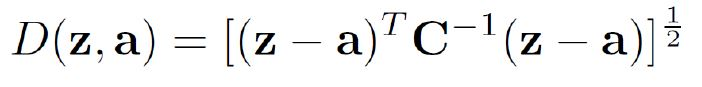
\includegraphics[scale=.5]{maha}
\end{itemize}

\item PROPOSED METHOD OF THE PAPER
\begin{itemize}
\item STEPS
\begin{enumerate}
\item Skin Color Region Segmentation
\item Binary Image Conversion
\item Noise Filtering
\item AdaBoost-Based Detector
\begin{enumerate}
\item Rectangular Features
\item Integral Image
\item AdaBoostAlgorithm

\end{enumerate}
\item Skin Color Range-Based Segmentation
\end{enumerate}
\end{itemize}

\item RESULT
\begin{enumerate}
\item Using skin color region to segment the face candidate does not necessarily reduce the detection time, and it is not always true that can improve the detection rate of the detector.
\item The performance of the detector is buffered by the AdaBoost-based detector.
\item When the range of mahalanobis distance increases not only detection increases the wrong faces are also increases.
\end{enumerate}
\end{itemize}
\item AKHIL A:
\begin{center}
\textbf{FACE DETECTION USING COMBINATION OF NEURAL NETWORK AND ADABOOST}

\end{center}

\begin{itemize}
\item INTRODUCTION
\begin{itemize}
\item This paper presents a combination of two wellknown algorithms, Adaboost
and Neural Network, to detect static images which is able to reduce the
false-positives drastically.
\item High false positive face detection is a crucial problem which leads to low
performance face recognition in surveillance system.
\item The performance can be increased by reducing these false positives so that
non-face can be discarded rst prior to recognition.
\item This method utilizes Haar-like features to extract theface rapidly using
integral image.
\item A cascade Adaboost classierS used to increase the face detection speed.
\item Due to using only this cascade Adaboost produces high false-positives, neural
network is used as the nal classier to verify face or non-face.
\item For a faster processing time, hierarchical Neural Network is used to increase
the face detection rate.
\end{itemize}
\item FACE DETECTION SYSTEM
\begin{itemize}
\item Face detection is the first step towards face recognition system
\item A decade of research, shows that most of the researchers use learning
machines for their face detection system because of its high performance and
reliability in real world applications
\item Most important in face detection system is a high accuracy and save
execution time.
\item Adaboost is good in detecting rate but contribute a lot of false detection rate.
But Neural Network has a good performance in facedetection but takes a
long time to process.
\end{itemize}
\item	SYSTEM ARCHITECTURE
\begin{itemize}
\item Figure illustrates our method which is a combination between cascade
adaboost and neural network as face's classifier.
\end{itemize}

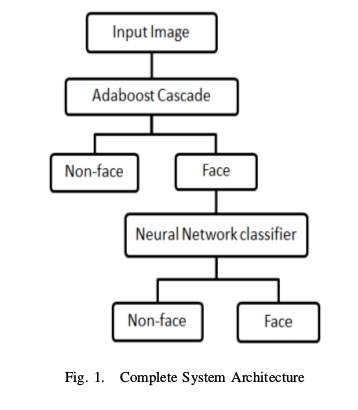
\includegraphics[scale=1]{akhil1}


\item	ADABOOST CASCADE CLASSIFIER
\begin{itemize}
\item Haar-like features as Box Classifier
\begin{itemize}
\item Haar Wavelets represented as box classifier which is used to extract face
features by using integral image.
\item There are 3 type of combination of box classifier which contains 14 templates
of Haar-like features in our training.
\item Here they areusing OpenCV as our Adaboost Classification task which has
a good performance in features extraction and face detection.
\end{itemize}
\end{itemize}
\item	NEURAL NETWORK CLASSIFIER
\begin{itemize}
\item In our proposed method, we use a simple type of neural network model which
is called Multi-Layer Feed-ForwardBackpropagation Network as our main part
in the second classifier.
\item Face candidates from Cascade Adaboost classier will be cropped and a
second classifier
\item Input image is added to reduce computation in search potential face
candidate in the search algorithm.Then, neural network task is to identify
nal output for the second classifier.
\end{itemize}

\end{itemize}
\newpage
\item ARAVIND RAVINDRAN
\begin{center}
\textbf{FAST TRAINING AND SELECTION OF HAAR FEATURES USING STATISTICS IN BOOSTING BASED FACE DETECTION}
\end{center}
\begin{itemize}
\item INTRODUCTION
\begin{itemize}
\item A standard image-based approach to face detection is scanning in raster order every squared sub-window of d pixels over multiple image scales
\item Then classify if each sub-window contains a face or not.
\item The strategy makes face detection a rare event binary classification problem
\item The node classifiers are constructed using an algorithm similar to AdaBoost
\item The algorithm combines an ensemble of weak classifiers to produce a final boosted classifier with very high accuracy.
\item The weak classifiers are typically trained from a discrete set of Haar features, which are rectangular Haar-like wavelets
\item Each feature is associated with a feature classifier, which classifies a sub-window by first integrating the sub-window with the feature’s
\end{itemize}

\item	OBSTACLE IN USE OF CASCADES
\begin{itemize}
\item Take a long time to train , even if all parameters are properly chosen.
\item The bottleneck is at training a weak classifier, of which the training time is O(N T log N ), where N is the number of examples used and T is the size of the feature set.
\item In practice,one has to run many trials and choose the best configuration,resulting in even longer training time.
\item Reducing N weakens the generalization, so reduce T by filtering the feature set and selecting only those discriminant for the current weak classifier
\end{itemize}

\item	LINEAR RELATIONSHIP BETWEEN IMAGE INTEGRAL AND FEATURE VALUE
\begin{itemize}
\item Let H (t) the matrix representing the t-th Haar-like wavelet w.r.t. the coordinate systemof the probed subwindow.
\item H (t) is a matrix of size d-by-d, of which the elements’ values are in a small discrete set.
\item Let v (t) the random variable representing the feature value observed from integrating the t-th Haar feature H (t) with a sub-window I. Let h (t) = H (t) , we get:\\
\begin{center}
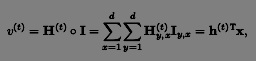
\includegraphics[scale=.7]{ara}
\end{center}

\end{itemize}
\end{itemize}
\item JITHIN S:
\begin{center}
\textbf{LEARNING BASED COMPUTER VISION WITH INTEL'S OPEN SOURCE COMPUTER VISION}
\end{center}
\begin{itemize}
\item OPEN SOURCE COMPUTER VISION LIBRARY
\begin{itemize}
\item Free open source collection of computer vision
\item Geared mainly towards human-computer interaction, robotics, security and other vision applications.
\item Open CV was designed for enablement and infrastructure
\item Open CV supports for vision is extensive. It supports routine for input, display, and storage of movies and single images.
\item Image processing is handled through convolution, thresholding, morphological operations, flood fills, histogramming, smoothing, pyramidal sub-sampling and a full suite of image algebra and arithmetic.
\item Open CV will automatically take advantage of and swap in the hand optimized in IPP providing a substantial speed-up to many vision routines.

\end{itemize}
\item FACE DETECTION
\begin{itemize}
\item The goals to find an object of a pre-defined class in a static image or video frame.
\item This task can be accomplished by extracting certain image features and then using some heuristics to find configurations and/or combination of those features specific to the object of interest.
\item In face detection it is complex to find heuristics that will handle the huge variety of instance of the object class.
\item For such objects, a statistical model(classifier) maybe trained instead and then used to detect the objects.
\end{itemize} 
\item STATISTICAL MODEL
\begin{itemize}
\item Takes multiple instances of object class of interest-positive or negative
\item They both makes a training set. During training different features are extracted from the training samples and distinctive features that can be used to classify the objects are selected.
\item The information is compressed into the statistical model parameters.
\item If the trained classifier does not detect an object or mistakenly detects the absent object, it is easy to make an adjustment by adding the corresponding positive or negative samples to the training set.
\item Open CV uses such a statistical approach for object detection. This method uses simple Haar-like features and a cascade of boosted tree classifiers as a statistical model.
\item The classifier is trained on images of fixed size and detection is done by sliding a search window of that size through the image and checking whether an image region at a certain location “looks like a face ” or not.
\item Each feature is described by the template its coordinate relative to the search window origin and the size of the feature.
\item Each feature consists of two or three joined “black” and “white” rectangles, either up-right or rotated 45 degree.
\end{itemize}
\end{itemize}
\item KIRAN TS
\begin{center}
\textbf{EMPIRICAL ANALYSIS OF DETECTION CASCADES OF BOOSTED CLASSIFIERS FOR RAPID OBJECT DETECTION}
\end{center}
\begin{itemize}


\item FEATURE POOL
\begin{itemize}
\item Let us assume that the basic unit for testing for the presence of an object is a window of W×H pixels.
\item Also assume that we have a very fast way of computing the sum of pixels of any upright and 45 degree rotated rectangle inside the window.
\begin{center}
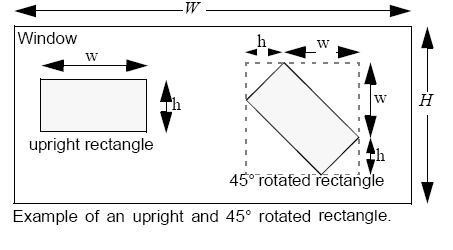
\includegraphics[scale=.5]{kira1}\\
\vspace{.2cm}
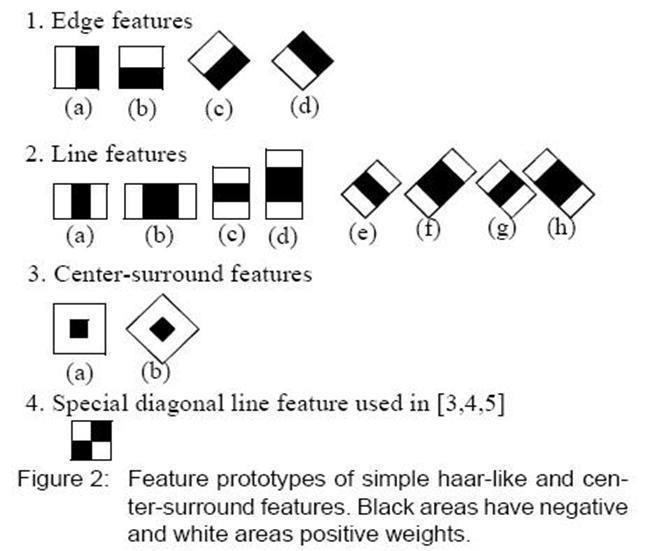
\includegraphics[scale=.5]{kira2}
\end{center}

\end{itemize}
\newpage
\item NUMBER OF FEATURE
\begin{itemize}
\item The number of features derived from each prototype is quite large and differs from prototype to prototype and can be calculated as follows:\\
\begin{center}
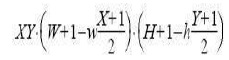
\includegraphics[scale=1]{kira3}
\end{center}
\item features for an image of size WxH, while a 45 degree rotated feature generates
\begin{center}
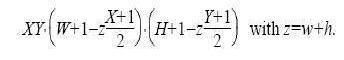
\includegraphics[scale=1]{kira4}
\end{center}
\end{itemize}
\item FAST FEATURE COMPUTATION
\begin{itemize}
\item A cascade of classifiers is a degenerated decision tree where at each stage a classifier is trained to detect almost all objects of interest while rejecting a certain fraction of the non-object patterns.
\item Each stage was trained to eliminated 50 percentage of the non-face patterns while falsely eliminating only 0.1 percentage of the frontal face patterns
\end{itemize}
\begin{center}
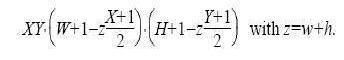
\includegraphics[scale=1]{kira4}
\end{center}

\end{itemize}

\end{enumerate}

\section{SAMPLE CODE}
\begin{tiny}
\begin{flushleft}
\begin{lstlisting}
package g7.blindsperceptron;

import java.io.File;
import java.io.FileOutputStream;
import java.io.IOException;
import java.io.InputStream;

import org.opencv.android.BaseLoaderCallback;
import org.opencv.android.CameraBridgeViewBase.CvCameraViewFrame;
import org.opencv.android.LoaderCallbackInterface;
import org.opencv.android.OpenCVLoader;
import org.opencv.core.Mat;
import org.opencv.core.MatOfRect;
import org.opencv.core.Rect;
import org.opencv.core.Scalar;
import org.opencv.core.Size;
import org.opencv.android.CameraBridgeViewBase;
import org.opencv.android.CameraBridgeViewBase.CvCameraViewListener2;
import org.opencv.objdetect.CascadeClassifier;
import org.opencv.imgproc.Imgproc;

import android.app.Activity;
import android.content.Context;
import android.os.Bundle;
import android.util.Log;
import android.view.WindowManager;

public class FdActivity extends Activity implements CvCameraViewListener2 {

    private static final String    TAG                 = "OCVSample::Activity";
    private static final Scalar    FACE_RECT_COLOR     = new Scalar(0, 255, 0, 255);
    public static final int        JAVA_DETECTOR       = 0;

    private Mat                    mRgba;
    private Mat                    mGray;
    private File                   mCascadeFile;
    private CascadeClassifier      mJavaDetector;

    private int                    mDetectorType       = JAVA_DETECTOR;
    private String[]               mDetectorName;

    private float                  mRelativeFaceSize   = 0.2f;
    private int                    mAbsoluteFaceSize   = 0;

    private CameraBridgeViewBase   mOpenCvCameraView;

    private BaseLoaderCallback  mLoaderCallback = new BaseLoaderCallback(this) {
        @Override
        public void onManagerConnected(int status) {
            switch (status) {
                case LoaderCallbackInterface.SUCCESS:
                {
                    Log.i(TAG, "OpenCV loaded successfully");
                    try {
                        // load cascade file from application resources
                        InputStream is = getResources().openRawResource(R.raw.lbpcascade_frontalface);
                        File cascadeDir = getDir("cascade", Context.MODE_PRIVATE);
                        mCascadeFile = new File(cascadeDir, "lbpcascade_frontalface.xml");
                        FileOutputStream os = new FileOutputStream(mCascadeFile);

                        byte[] buffer = new byte[4096];
                        int bytesRead;
                        while ((bytesRead = is.read(buffer)) != -1) {
                            os.write(buffer, 0, bytesRead);
                        }
                        is.close();
                        os.close();

                        mJavaDetector = new CascadeClassifier(mCascadeFile.getAbsolutePath());
                        if (mJavaDetector.empty()) {
                            Log.e(TAG, "Failed to load cascade classifier");
                            mJavaDetector = null;
                        } else
                            Log.i(TAG, "Loaded cascade classifier from " + mCascadeFile.getAbsolutePath());


                        cascadeDir.delete();

                    } catch (IOException e) {
                        e.printStackTrace();
                        Log.e(TAG, "Failed to load cascade. Exception thrown: " + e);
                    }

                    mOpenCvCameraView.enableView();
                } break;
                default:
                {
                    super.onManagerConnected(status);
                } break;
            }
        }
    };

    public FdActivity() {
        mDetectorName = new String[2];
        mDetectorName[JAVA_DETECTOR] = "Java";

        Log.i(TAG, "Instantiated new " + this.getClass());
    }

    /** Called when the activity is first created. */
    @Override
    public void onCreate(Bundle savedInstanceState) {
        Log.i(TAG, "called onCreate");
        super.onCreate(savedInstanceState);
        getWindow().addFlags(WindowManager.LayoutParams.FLAG_KEEP_SCREEN_ON);

        setContentView(R.layout.face_detect_surface_view);

        mOpenCvCameraView = (CameraBridgeViewBase) findViewById(R.id.fd_activity_surface_view);
        mOpenCvCameraView.setCvCameraViewListener(this);

    }

    @Override
    public void onPause()
    {
        super.onPause();
        if (mOpenCvCameraView != null)
            mOpenCvCameraView.disableView();
    }

    @Override
    public void onResume()
    {
        super.onResume();
        if (!OpenCVLoader.initDebug()) {
            Log.d(TAG, "Internal OpenCV library not found. Using OpenCV Manager for initialization");
            OpenCVLoader.initAsync(OpenCVLoader.OPENCV_VERSION_3_0_0, this, mLoaderCallback);
        } else {
            Log.d(TAG, "OpenCV library found inside package. Using it!");
            mLoaderCallback.onManagerConnected(LoaderCallbackInterface.SUCCESS);
        }
    }

    public void onDestroy() {
        super.onDestroy();
        mOpenCvCameraView.disableView();
    }

    public void onCameraViewStarted(int width, int height) {
        mGray = new Mat();
        mRgba = new Mat();
    }

    public void onCameraViewStopped() {
        mGray.release();
        mRgba.release();
    }

    public Mat onCameraFrame(CvCameraViewFrame inputFrame) {

        mRgba = inputFrame.rgba();
        mGray = inputFrame.gray();

        if (mAbsoluteFaceSize == 0) {
            int height = mGray.rows();
            if (Math.round(height * mRelativeFaceSize) > 0) {
                mAbsoluteFaceSize = Math.round(height * mRelativeFaceSize);
            }

	        }

        MatOfRect faces = new MatOfRect();

        if (mDetectorType == JAVA_DETECTOR) {
            if (mJavaDetector != null)
                mJavaDetector.detectMultiScale(mGray, faces, 1.1, 2, 2, // TODO: objdetect.CV_HAAR_SCALE_IMAGE
                        new Size(mAbsoluteFaceSize, mAbsoluteFaceSize), new Size());
        }
        else {
            Log.e(TAG, "Detection method is not selected!");
        }

        Rect[] facesArray = faces.toArray();
        for (int i = 0; i < facesArray.length; i++)
            Imgproc.rectangle(mRgba, facesArray[i].tl(), facesArray[i].br(), FACE_RECT_COLOR, 3);

        return mRgba;
    }

}

\end{lstlisting}


\end{flushleft}
\end{tiny}
\newpage
\section{PROGRAM FLOW EXPLANATION}
\paragraph{ }
An activity is a single, focused thing that the user can do. Almost all activities interact with the user, so the Activity class takes care of creating a window for you in which you can place your UI with setContentView(View). Activity life cycle of android is given by
\begin{figure}[htpb]

\begin{center}
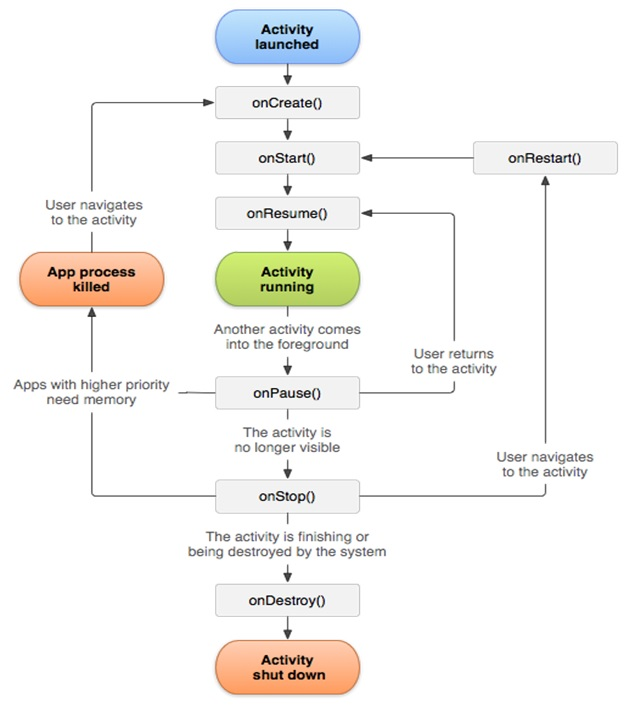
\includegraphics[scale=.6]{analysis}
\caption{Activity life cycle}

\end{center}
\end{figure}
\paragraph{ }In our code we imported the following functionalities using OpenCV library.
\begin{enumerate}
\item Cascade Classifier
\item Camera view frame
\item Image processing library for draw rectangles.

\end{enumerate}
\begin{flushleft}

import org.opencv.android.BaseLoaderCallback;\\
import org.opencv.android.CameraBridgeViewBase.CvCameraViewFrame;\\
import org.opencv.android.LoaderCallbackInterface;\\
import org.opencv.android.OpenCVLoader;\\
import org.opencv.core.Mat;\\
import org.opencv.core.MatOfRect;\\
import org.opencv.core.Rect;\\
import org.opencv.core.Scalar;\\
import org.opencv.core.Size;\\
import org.opencv.android.CameraBridgeViewBase;\\
import org.opencv.android.CameraBridgeViewBase.CvCameraViewListener2;

import org.opencv.objdetect.CascadeClassifier;\\
import org.opencv.imgproc.Imgproc;\\

\vspace{.3cm}

And then we created a object of CascadeClassifier    named mJavaDetector.
All the necessary objects like org.opencv.core.Mat, org.opencv.core.MatOfRect,..etc are declared.

\vspace{.4cm}
\textbf{
The onCreate() method
}
\end{flushleft}

\paragraph{ }Here the Activity initialization is done and content which is to be displayed is called. And the Camera started to listen for faces.

\begin{small}

\begin{lstlisting}
@Override
public void onCreate(Bundle savedInstanceState) {
Log.i(TAG, "called onCreate");
Super.onCreate(savedInstanceState);
getWindow().addFlags(WindowManager.LayoutParams.FLAG_KEEP_SCREEN_ON);
setContentView(R.layout.face_detect_surface_view);

mOpenCvCameraView = (CameraBridgeViewBase) findViewById(R.id.fd_activity_surface_view);
mOpenCvCameraView.setCvCameraViewListener(this);

}
\end{lstlisting}


\end{small}

\vspace{.3cm}
\begin{flushleft}
\textbf{OnManagerConnected(int status) method}\\

\end{flushleft}

Here all the opencv package libraries are loaded into local class file.
\begin{flushleft}
\begin{small}
\begin{lstlisting}
private BaseLoaderCallback  mLoaderCallback = new BaseLoaderCallback(this) {
@Override
public void onManagerConnected(int status) {
  switch (status) {
  case LoaderCallbackInterface.SUCCESS:
  {
        Log.i(TAG, "OpenCV loaded successfully");
        try {
            // load cascade file from application resources
         InputStream is = getResources().openRawResource(R.raw.lbpcascade_frontalface);
         File cascadeDir = getDir("cascade", Context.MODE_PRIVATE);
          mCascadeFile = new File(cascadeDir, "lbpcascade_frontalface.xml");
          FileOutputStream os = new FileOutputStream(mCascadeFile);

               byte[] buffer = new byte[4096];
               int bytesRead;
               while ((bytesRead = is.read(buffer)) != -1) {
               os.write(buffer, 0, bytesRead);
             }
             is.close();
             os.close();

         mJavaDetector = new CascadeClassifier(mCascadeFile.getAbsolutePath());
         if (mJavaDetector.empty()) {
         Log.e(TAG, "Failed to load cascade classifier");
         mJavaDetector = null;
       } else
 Log.i(TAG, "Loaded cascade classifier from " + mCascadeFile.getAbsolutePath());


           cascadeDir.delete();

      } catch (IOException e) {
             e.printStackTrace();
             Log.e(TAG, "Failed to load cascade. Exception thrown: " + e);
    }

    mOpenCvCameraView.enableView();
 } break;
   default:
   {
      super.onManagerConnected(status);
   } break;
 }
}
};

\end{lstlisting}
\end{small}
\end{flushleft}
%=\vspace{.1cm}
\begin{flushleft}
\textbf{OnCameraViewStopped() method}\\

\end{flushleft}
\paragraph{ }Here the two Mat variables are released.

\begin{flushleft}
\begin{flushleft}

\end{flushleft}
public void onCameraViewStopped() {\\
    mGray.release();\\
    mRgba.release();\\
}
\end{flushleft}

\newpage
\begin{flushleft}
\textbf{OnCameraFrame(CvCameraViewFrame inputFrame)method}
\end{flushleft}
\paragraph{ }Here on each frame if the frame contain face features it is identified using HAAR classifier in open cv library. And if the face is detected using imgproc a rectangle is drawn.
\begin{flushleft}
\begin{tiny}
\begin{lstlisting}
public Mat onCameraFrame(CvCameraViewFrame inputFrame) {

    mRgba = inputFrame.rgba();
    mGray = inputFrame.gray();

    if (mAbsoluteFaceSize == 0) {
        int height = mGray.rows();
        if (Math.round(height * mRelativeFaceSize) > 0) {
            mAbsoluteFaceSize = Math.round(height * mRelativeFaceSize);
        }

    }

    MatOfRect faces = new MatOfRect();

    if (mDetectorType == JAVA_DETECTOR) {
        if (mJavaDetector != null)
            mJavaDetector.detectMultiScale(mGray, faces, 1.1, 2, 2, // TODO: objdetect.CV_HAAR_SCALE_IMAGE
                    new Size(mAbsoluteFaceSize, mAbsoluteFaceSize), new Size());
    }
    else {
        Log.e(TAG, "Detection method is not selected!");
    }

    Rect[] facesArray = faces.toArray();
    for (int i = 0; i < facesArray.length; i++)
        Imgproc.rectangle(mRgba, facesArray[i].tl(), facesArray[i].br(), FACE_RECT_COLOR, 3);

    return mRgba;
}

\end{lstlisting}
\end{tiny}
\end{flushleft}

\section{PROJECT SUMMARY}
\paragraph{ }The blind can only get perceptive and audio information, which bring them huge barriers to action. Mobile devices could provide the blind great help.
Here the project presents a system which uses neural network for face recognition, which widely provides the blind user to identify the person in-front of him. Also the  project provides a system to navigate the blind, detect the obstacles in-front of him, provides instruction for easier navigation.

\section{PROJECT DIARY}
\begin{flushleft}

\textbf{August 11/2015}\\
\begin{itemize}
\item Topic selection
\begin{itemize}
\item Topic "Blind Navigation using ultrasonic sensors and Image recognition" was sent.
\item New Topic was Assigned.
\item "Guidance Perfomance Analsis for Blind navigation System Using Neural learnig image recognition system"

\item Abstract and base paper of the project are sent.
\end{itemize}
\end{itemize}
\textbf{September 17/2015}\\
\begin{itemize}
\item Presentation Slides prepared for each reference papers were sent\\

\item Work allocated among group members
\end{itemize}
\textbf{September 26/2015}\\
\begin{itemize}
\item Submitted Literature review for refernce papers
\end{itemize}
\textbf{
October 06/2015}\\
\begin{itemize}
\item Presentd papares by
\begin{itemize}
\item AJITHKUMAR AK
\item AKHIL A
\item ARAVIND RAVINDRAN
\item JITHIN S
\item KIRAN TS
\end{itemize}
\end{itemize}
\textbf{December 20/2015}\\
\begin{itemize}
\item Configured android studio sdk
\end{itemize}
\textbf{December 31/2015}
\begin{itemize}
\item Added open cv dependancy on to the applicaiton.
\end{itemize}
\newpage
\textbf{january 3/2016}
\begin{itemize}
\item Started coding..
\item Refreshed UI and created hello world on studio and run on Machine.

\end{itemize}
\textbf{January 6/2013}
\begin{itemize}
\item Started creating our project
\begin{itemize}
\item Imported old source codes and configured..
\end{itemize}
\end{itemize}

\textbf{January 13/2013}
\begin{itemize}
\item Sample code is verified by guide

\end{itemize}
 

\end{flushleft}
\section{SUGGESTION TO READERS}
\begin{itemize}
\item Readers should have basic idea about android programming, Image processing , smart phone basics.
\item Readers should have basic idea about Neural Network.
\item Readers are advised to have knowledge about face recognition system.
\item various techniques are used for the identification of an individual using some machine learning techniques.
\item More better advancements are done to each step of development to enhance the system.
\end{itemize}

\end{appendix}
\end{document}